\section{Executable Evaluation}
\label{sec:evaluation}

We evaluate numerical correctness, declared model behavior, and application
contracts separately. All learner outcomes in the numerical report are
synthetic. None were loaded into the live interface as user history.
The canonical record is
\artifact{docs/learner-evaluation/results.json}; its Markdown companion,
figures, and this paper's numerical macros are generated from the same file.
The default experiment seed is 140015. Fits use two chains, 384 warm-up
iterations, and 256 retained draws per chain unless the reference experiment
specifies otherwise.

\subsection{Independent Numerical Reference}

A one-dimensional submodel removes unrelated effects and dynamics, sets
the memory-logit prior to standard normal, and supplies eight successes and
two failures. Composite Simpson integration on a bounded logit interval
provides an independent reference for the response probability posterior.
This is a useful test because it evaluates a known density by a different
numerical method, rather than checking the sampler against its own update
equations.

The numerical reference mean is \LearnerReferenceMean{}; the sampled mean is
\LearnerSampledMean{}, an absolute difference of \LearnerReferenceError{}.
The report also compares the 5th and 95th percentiles. Numerical acceptance
tolerances are specified before the generated report: 0.025 for the mean and
0.06 for each interval endpoint. These are implementation tolerances, not
confidence levels or human calibration guarantees. A separate unit test
integrates a normal--inverse-Gamma submodel to check learned variance
inference, including its conditional conjugacy.

\subsection{Declared Sharing and Local Counterevidence}

We fit the actual authored contextual-reading tasks for the aligned
written-text reading in Arabic, Spanish, and English, alongside an unobserved
Spanish exceptional-form recall task. The first evidence condition contains
21 correct answers among 24 Arabic responses in separate synthetic episodes.
The second adds 18 incorrect Spanish reading responses. Dynamics are disabled
in this comparison, so changing dates cannot explain changes in predictions.

\begin{figure*}[t]
\centering
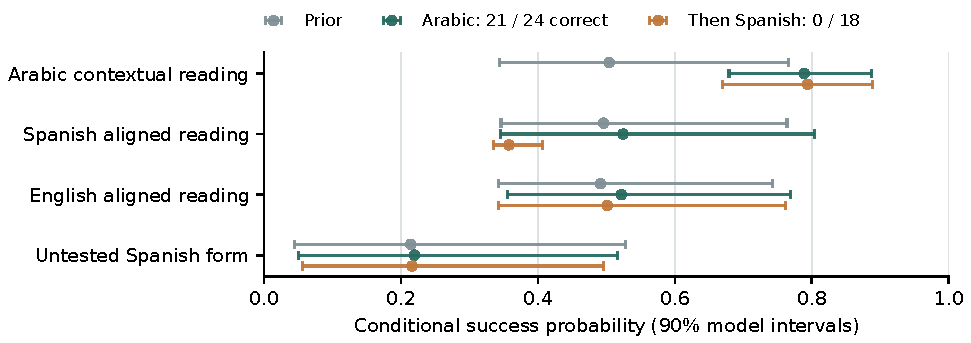
\includegraphics[width=.96\textwidth]{figures/learner_transfer.pdf}
\caption{Actual posterior predictions under three synthetic evidence
conditions. Points are means and horizontal lines are 90\% model intervals.
The Arabic responses inform a declared shared reading, while local lexical
effects and untested forms remain uncertain. Spanish counterevidence can
defeat the initial borrowed prediction. Differences among untouched
prior-only draws across independently seeded fits are Monte Carlo variation,
not learned foreign vocabulary.}
\label{fig:transfer}
\end{figure*}

The Arabic mean changes from \LearnerArabicPrior{} to
\LearnerArabicPosterior{}. The Spanish aligned-reading mean after Arabic
evidence is \LearnerSpanishBorrowed{}, with a broad interval; after its own
counterevidence it is \LearnerSpanishCounter{}. The unobserved Spanish
exceptional form remains prior-only, with mean \LearnerUntestedForm{}
after the Arabic evidence. Figure~\ref{fig:transfer} makes the distinction
between a shared reading and local word-form knowledge visible.

The Spanish all-failure condition is deliberately adverse. Because the
authored recognition task has a fixed guessing floor, its predicted success
cannot approach zero. This exposes a substantive likelihood assumption:
systematic mistakes and distractor preferences may require a different
response model. The experiment checks that local evidence is not erased by
pooling; it is not an estimate of negative transfer between human languages.

A separately generated sequence of 64 Bernoulli outcomes, with stipulated
success probability 0.85, has 59 successes under the fixed seed. On this one
sequence, the prior and updated Arabic predictions have Brier scores
\LearnerBrierPrior{} and \LearnerBrierPosterior{}, and log losses
\LearnerLogPrior{} and \LearnerLogPosterior{}. These proper scores describe
the supplied example. They do not establish superiority to knowledge tracing,
item-response models, or existing repetition systems, and they do not
constitute a cross-learner calibration study.

\subsection{Decision Arithmetic and a Fitted Example}

The decision module is tested against \LearnerExactCases{} hand-computable
finite-posterior cases. The basic case assigns equal probability to a root
gap and a pattern gap. Each corresponding support costs 0.2, and an ideal
diagnostic costs 0.1. Acting without information has risk 0.7; a diagnostic
followed by the appropriate support has risk 0.3. Information value is 0.5
and net improvement is 0.4. A noisy diagnostic with outcome probabilities
0.8 and 0.2 has information value 0.3 and net improvement 0.2.

\begin{figure*}[t]
\centering
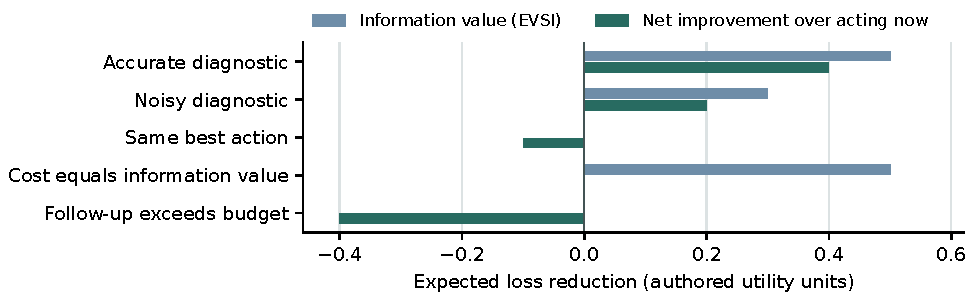
\includegraphics[width=.96\textwidth]{figures/learner_decisions.pdf}
\caption{Hand-computable cases evaluated by the shipped policy. Information
value is separated from net improvement after effort, delay, and remaining
budget. A question with an informative answer can have zero decision value
when the same support remains optimal. A positive information value can also
be insufficient to justify its cost. These are exact synthetic decision
checks, not measured learner benefits.}
\label{fig:decisions}
\end{figure*}

Other cases cover an uninformative question, an informative question whose
outcomes share the same best action, a known gap, break-even cost, a diagnostic
that consumes the follow-up support budget, and an explicit no-practice
constraint. All \LearnerExactCases{} cases pass. Additional tests preserve
covariance when multiple targets share joint posterior draws, reject
unsupported component bypasses, honor nonuniform weights, and fail safely
when a total computation bound is exceeded.

The report also sends a fitted posterior into the same policy.
Its synthetic history contains 20 successful Arabic base-recall responses
and 20 unsuccessful responses on a different lexical base with the relevant
Arabic pattern. The lowest-loss action supplies the authored pattern cue.
The full report retains its candidate losses and diagnostic outcome branches,
so this result can be inspected without inferring a diagnosis from the action
name alone.

\subsection{Temporal and Application Verification}

A separate dynamic fit predicts a lower success probability after 30 days
without an additional accepted opportunity. This checks the implemented
nonnegative decay term. It does not establish a measured forgetting curve.
Tests also cover disabled dynamics, mode separation, explicit cohort
authorization, task and parameter caps, deterministic replay, and
asynchronous cancellation.

The release's verification run includes \LearnerNodeTests{} passing
JavaScript unit tests, \LearnerDOMTests{} passing executable DOM/integration
tests, and \LearnerAPITests{} passing Python tests. The latter include the
actual new task's scorer and analysis references round-tripping through
FastAPI and SQLite. The application tests execute the shipping self-contained
HTML, select a goal, answer a task, recompute a posterior and decision, and
export the scoped calculation. They check that unrelated cards, schedules,
and reader content are preserved.

Cross-task exposure tests are particularly consequential. They verify
recognition-prompt to recall leakage, supplied-base to base-recall leakage,
an exceptional form shown under one task ID and answered under another,
same-form repetition, recorded component hints, future and expired exposures, and account/team
separation. The bridge independently reconciles these exposures for imported
events; it does not trust the UI alone. A response's own later feedback
cannot invalidate it retrospectively.

The full native-browser visual run was blocked because the execution
environment denied Chromium's socket creation. No claim is made here about
native-browser layout, real assistive technology, or native IndexedDB
durability. The DOM transaction fixture, actual server persistence tests,
source inspection, and compiled-bundle execution are distinct forms of
coverage, and the verification record states which were run.

\paragraph{Runtime.}
The saved numerical suite reports \LearnerRuntime{} milliseconds on its
recorded Node/Linux environment. This is a measured run of the bounded
synthetic cases, not a service-level guarantee or a benchmark on mobile
hardware. All candidate, observation, coefficient, sampling, and decision-work
limits are inspectable in source. Asynchronous fitting yields so the user can
continue or change context.

\section{Limits and Next Empirical Questions}

\paragraph{Linguistic and measurement validity.}
The 93 new tasks are a small authored slice. Richer morphology is bounded
to the declared Arabic, English, and Spanish examples; the remaining language
coverage consists of two vocabulary items in two response modes. All are
labelled authored and not independently instructor-reviewed. Dialect,
register, productive composition, phonological competence, valid alternative
answers, and task instruction comprehension require further work. Exact
answer matching measures the declared rubric, which can be narrower than
linguistic correctness.

\paragraph{Statistical limitations.}
The full decomposition is not generally identified by available responses.
Root, language, word, context, memory, and time effects can explain similar
patterns. Learned variances remain prior-sensitive, especially with few
groups. The shared-factor design expresses positive common variation, not an
arbitrary learned covariance or a causal transfer mechanism. Guessing,
lapses, difficulty offsets, and supported-component behavior are currently
authored settings. History truncation is reported and can change fitted
temporal covariates. Lightweight predictive diagnostics do not certify that
every latent quantity is well mixed.

\paragraph{Decision limitations.}
The implemented policy chooses one diagnostic followed by one terminal
action. Its loss concerns immediate completion, and its support model assumes
the declared cue supplies a component. That may be useful as an operational
assumption, but it requires empirical assessment. Long-horizon teaching,
retained learning, motivation, frustration, and opportunity costs beyond the
chosen task are not optimized. Observational practice trends are not
substituted for intervention effects. The user can always continue or choose
an optional task directly.

\paragraph{Evaluation needed for educational claims.}
A defensible human study would first review task content and rubrics, then
evaluate held-out task prediction with learner and item splits, compare
pooling structures and simpler baselines, inspect calibration by language and
response mode, and assess sensitivity to prior and nuisance settings.
Intervention claims require assignment or another justified causal design,
with delayed outcomes and interruption costs measured separately. The
present artifact makes those experiments implementable and auditable; their
results are not supplied by its graph or by successful software tests.

\section{Conclusion}

\Nabu{} 1.15.0 implements a concrete path from versioned task observations to
a hierarchical learner posterior and an actionable Bayesian decision.
Required ingredients, whole-form memory, explicit shared meanings, local
lexical forms, response modes, and time remain distinguishable in the model.
The decision calculation values information through its effect on available
actions. Its tests establish numerical and integration properties within
declared assumptions, while preserving the empirical questions that require
human evidence.
